\documentclass[mstat,12pt]{unswthesis}
\usepackage[a4paper,margin=2.5cm]{geometry}

\usepackage{color}
\usepackage{fancyvrb}
\newcommand{\VerbBar}{|}
\newcommand{\VERB}{\Verb[commandchars=\\\{\}]}
\DefineVerbatimEnvironment{Highlighting}{Verbatim}{commandchars=\\\{\}}
% Add ',fontsize=\small' for more characters per line
\usepackage{framed}
\definecolor{shadecolor}{RGB}{248,248,248}
\newenvironment{Shaded}{\begin{snugshade}}{\end{snugshade}}
\newcommand{\AlertTok}[1]{\textcolor[rgb]{0.94,0.16,0.16}{#1}}
\newcommand{\AnnotationTok}[1]{\textcolor[rgb]{0.56,0.35,0.01}{\textbf{\textit{#1}}}}
\newcommand{\AttributeTok}[1]{\textcolor[rgb]{0.13,0.29,0.53}{#1}}
\newcommand{\BaseNTok}[1]{\textcolor[rgb]{0.00,0.00,0.81}{#1}}
\newcommand{\BuiltInTok}[1]{#1}
\newcommand{\CharTok}[1]{\textcolor[rgb]{0.31,0.60,0.02}{#1}}
\newcommand{\CommentTok}[1]{\textcolor[rgb]{0.56,0.35,0.01}{\textit{#1}}}
\newcommand{\CommentVarTok}[1]{\textcolor[rgb]{0.56,0.35,0.01}{\textbf{\textit{#1}}}}
\newcommand{\ConstantTok}[1]{\textcolor[rgb]{0.56,0.35,0.01}{#1}}
\newcommand{\ControlFlowTok}[1]{\textcolor[rgb]{0.13,0.29,0.53}{\textbf{#1}}}
\newcommand{\DataTypeTok}[1]{\textcolor[rgb]{0.13,0.29,0.53}{#1}}
\newcommand{\DecValTok}[1]{\textcolor[rgb]{0.00,0.00,0.81}{#1}}
\newcommand{\DocumentationTok}[1]{\textcolor[rgb]{0.56,0.35,0.01}{\textbf{\textit{#1}}}}
\newcommand{\ErrorTok}[1]{\textcolor[rgb]{0.64,0.00,0.00}{\textbf{#1}}}
\newcommand{\ExtensionTok}[1]{#1}
\newcommand{\FloatTok}[1]{\textcolor[rgb]{0.00,0.00,0.81}{#1}}
\newcommand{\FunctionTok}[1]{\textcolor[rgb]{0.13,0.29,0.53}{\textbf{#1}}}
\newcommand{\ImportTok}[1]{#1}
\newcommand{\InformationTok}[1]{\textcolor[rgb]{0.56,0.35,0.01}{\textbf{\textit{#1}}}}
\newcommand{\KeywordTok}[1]{\textcolor[rgb]{0.13,0.29,0.53}{\textbf{#1}}}
\newcommand{\NormalTok}[1]{#1}
\newcommand{\OperatorTok}[1]{\textcolor[rgb]{0.81,0.36,0.00}{\textbf{#1}}}
\newcommand{\OtherTok}[1]{\textcolor[rgb]{0.56,0.35,0.01}{#1}}
\newcommand{\PreprocessorTok}[1]{\textcolor[rgb]{0.56,0.35,0.01}{\textit{#1}}}
\newcommand{\RegionMarkerTok}[1]{#1}
\newcommand{\SpecialCharTok}[1]{\textcolor[rgb]{0.81,0.36,0.00}{\textbf{#1}}}
\newcommand{\SpecialStringTok}[1]{\textcolor[rgb]{0.31,0.60,0.02}{#1}}
\newcommand{\StringTok}[1]{\textcolor[rgb]{0.31,0.60,0.02}{#1}}
\newcommand{\VariableTok}[1]{\textcolor[rgb]{0.00,0.00,0.00}{#1}}
\newcommand{\VerbatimStringTok}[1]{\textcolor[rgb]{0.31,0.60,0.02}{#1}}
\newcommand{\WarningTok}[1]{\textcolor[rgb]{0.56,0.35,0.01}{\textbf{\textit{#1}}}}


%%%%%%%%%%%%%%%%%%%%%%%%%%%%%%%%%%%%%%%%%%%%%%%%%%%%%%%%%%%%%%%%%%
% 
% OK...Now we get to some actual input.  The first part sets up
% the title etc that will appear on the front page
%
%%%%%%%%%%%%%%%%%%%%%%%%%%%%%%%%%%%%%%%%%%%%%%%%%%%%%%%%%%%%%%%%%

\title{Projet réalisé par\\[0.5cm] l'équipe InvestigationData du groupe de TD2 \\[3cm]Rapport
de groupe des UE \newline  Bases de données + Sciences des Données 2}

\authornameonly{Abbassi Younes, Allaali Narjis, Bouguima
Kawthar, Taghnakt Myriam }

\author{\Authornameonly}

\copyrightfalse
\figurespagefalse
\tablespagefalse

%%%%%%%%%%%%%%%%%%%%%%%%%%%%%%%%%%%%%%%%%%%%%%%%%%%%%%%%%%%%%%%%%
%
%  And now the document begins
%  The \beforepreface and \afterpreface commands puts the
%  contents page etc in
%
%%%%%%%%%%%%%%%%%%%%%%%%%%%%%%%%%%%%%%%%%%%%%%%%%%%%%%%%%%%%%%%%%%


%%%%%%%%%%%%%%%%%%%%%%%%%%%%%%%%%%%%%%%%%%%%%%%%%%%%%%%%%%%%%%%%%%%%%%%
%
%  A small sample UNSW Coursework Masters thesis file.
%  Any questions to Ian Doust i.doust@unsw.edu.au and/or Gery Geenens ggeenens@unsw.edu.au
%
%%%%%%%%%%%%%%%%%%%%%%%%%%%%%%%%%%%%%%%%%%%%%%%%%%%%%%%%%%%%%%%%%%%%%%%
%
%  The first part pulls in a UNSW Thesis class file.  This one is
%  slightly nonstandard and has been set up to do a couple of
%  things automatically
%
 
%%%%%%%%%%%%%%%%%
%% Precisely one of the next four lines should be uncommented.
%% Choose the one which matches your degree, uncomment it, and comment out the other two!
%\documentclass[mfin,12pt]{unswthesis}    %%  For Master of Financial Mathematics 
%\documentclass[mmath,12pt]{unswthesis}   %%  For Master of Mathematics
%\documentclass[mstat,12pt]{unswthesis}  %%  For Master of Statistics
%%%%%%%%%%%%%%%%%



\linespread{1}
%marge

\usepackage{amsfonts}
\usepackage{amssymb}
\usepackage{amsthm}
\usepackage{latexsym,amsmath}
\usepackage{graphicx}
\usepackage{afterpage}
\usepackage[colorlinks]{hyperref}
 \hypersetup{
     colorlinks=true,
     linkcolor=blue,
     filecolor=blue,
     citecolor= black,      
     urlcolor=cyan,
     }
\usepackage{textcomp}
\usepackage{longtable}
\usepackage{booktabs}
\usepackage{float}
\let\origfigure\figure
\let\endorigfigure\endfigure
\renewenvironment{figure}[1][2] {
    \expandafter\origfigure\expandafter[H]
} {
    \endorigfigure
}
\usepackage[T1]{fontenc}
\usepackage{ragged2e}
\def\tightlist{}
\usepackage[french]{babel}

%fonctionnement tableau
\usepackage{array}
\usepackage{calc}

%%%%%%%%%%%%%%%%%%%%%%%%%%%%%%%%%%%%%%%%%%%%%%%%%%%%%%%%%%%%%%%%%
%
%  The following are some simple LaTeX macros to give some
%  commonly used letters in funny fonts. You may need more or less of
%  these
%
\newcommand{\R}{\mathbb{R}}
\newcommand{\Q}{\mathbb{Q}}
\newcommand{\C}{\mathbb{C}}
\newcommand{\N}{\mathbb{N}}
\newcommand{\F}{\mathbb{F}}
\newcommand{\PP}{\mathbb{P}}
\newcommand{\T}{\mathbb{T}}
\newcommand{\Z}{\mathbb{Z}}
\newcommand{\B}{\mathfrak{B}}
\newcommand{\BB}{\mathcal{B}}
\newcommand{\M}{\mathfrak{M}}
\newcommand{\X}{\mathfrak{X}}
\newcommand{\Y}{\mathfrak{Y}}
\newcommand{\CC}{\mathcal{C}}
\newcommand{\E}{\mathbb{E}}
\newcommand{\cP}{\mathcal{P}}
\newcommand{\cS}{\mathcal{S}}
\newcommand{\A}{\mathcal{A}}
\newcommand{\ZZ}{\mathcal{Z}}
%%%%%%%%%%%%%%%%%%%%%%%%%%%%%%%%%%%%%%%%%%%%%%%%%%%%%%%%%%%%%%%%%%%%%
%
% The following are much more esoteric commands that I have left in
% so that this file still processes. Use or delete as you see fit
%
\newcommand{\bv}[1]{\mbox{BV($#1$)}}
\newcommand{\comb}[2]{\left(\!\!\!\begin{array}{c}#1\\#2\end{array}\!\!\!\right)
}
\newcommand{\Lat}{{\rm Lat}}
\newcommand{\var}{\mathop{\rm var}}
\newcommand{\Pt}{{\mathcal P}}
\def\tr(#1){{\rm trace}(#1)}
\def\Exp(#1){{\mathbb E}(#1)}
\def\Exps(#1){{\mathbb E}\sparen(#1)}
\newcommand{\floor}[1]{\left\lfloor #1 \right\rfloor}
\newcommand{\ceil}[1]{\left\lceil #1 \right\rceil}
\newcommand{\hatt}[1]{\widehat #1}
\newcommand{\modeq}[3]{#1 \equiv #2 \,(\text{mod}\, #3)}
\newcommand{\rmod}{\,\mathrm{mod}\,}
\newcommand{\p}{\hphantom{+}}
\newcommand{\vect}[1]{\mbox{\boldmath $ #1 $}}
\newcommand{\reff}[2]{\ref{#1}.\ref{#2}}
\newcommand{\psum}[2]{\sum_{#1}^{#2}\!\!\!'\,\,}
\newcommand{\bin}[2]{\left( \begin{array}{@{}c@{}}
				#1 \\ #2
			\end{array}\right)	}
%
%  Macros - some of these are in plain TeX (gasp!)
%
\newcommand{\be}{($\beta$)}
\newcommand{\eqp}{\mathrel{{=}_p}}
\newcommand{\ltp}{\mathrel{{\prec}_p}}
\newcommand{\lep}{\mathrel{{\preceq}_p}}
\def\brack#1{\left \{ #1 \right \}}
\def\bul{$\bullet$\ }
\def\cl{{\rm cl}}
\let\del=\partial
\def\enditem{\par\smallskip\noindent}
\def\implies{\Rightarrow}
\def\inpr#1,#2{\t \hbox{\langle #1 , #2 \rangle} \t}
\def\ip<#1,#2>{\langle #1,#2 \rangle}
\def\lp{\ell^p}
\def\maxb#1{\max \brack{#1}}
\def\minb#1{\min \brack{#1}}
\def\mod#1{\left \vert #1 \right \vert}
\def\norm#1{\left \Vert #1 \right \Vert}
\def\paren(#1){\left( #1 \right)}
\def\qed{\hfill \hbox{$\Box$} \smallskip}
\def\sbrack#1{\Bigl \{ #1 \Bigr \} }
\def\ssbrack#1{ \{ #1 \} }
\def\smod#1{\Bigl \vert #1 \Bigr \vert}
\def\smmod#1{\bigl \vert #1 \bigr \vert}
\def\ssmod#1{\vert #1 \vert}
\def\sspmod#1{\vert\, #1 \, \vert}
\def\snorm#1{\Bigl \Vert #1 \Bigr \Vert}
\def\ssnorm#1{\Vert #1 \Vert}
\def\sparen(#1){\Bigl ( #1 \Bigr )}

\newcommand\blankpage{%
    \null
    \thispagestyle{empty}%
    \addtocounter{page}{-1}%
    \newpage}

%%%%%%%%%%%%%%%%%%%%%%%%%%%%%%%
%
% These environments allow you to get nice numbered headings
%  for your Theorems, Definitions etc.  
%
%  Environments
%
%%%%%%%%%%%%%%%%%%%%%%%%%%%%%%%

\newtheorem{theorem}{Theorem}[section]
\newtheorem{lemma}[theorem]{Lemma}
\newtheorem{proposition}[theorem]{Proposition}
\newtheorem{corollary}[theorem]{Corollary}
\newtheorem{conjecture}[theorem]{Conjecture}
\newtheorem{definition}[theorem]{Definition}
\newtheorem{example}[theorem]{Example}
\newtheorem{remark}[theorem]{Remark}
\newtheorem{question}[theorem]{Question}
\newtheorem{notation}[theorem]{Notation}
\numberwithin{equation}{section}

%%%%%%%%%%%%%%%%%%%%%%%%%%%%%%%%%%%%%%%%%%%%%%%%%%%%%%%%%%%%%%%%%%
%
%  If you've got some funny special words that LaTeX might not
% hyphenate properly, you can give it a helping hand:
%

\hyphenation{Mar-cin-kie-wicz Rade-macher}


\newlength{\cslhangindent}
\setlength{\cslhangindent}{1.5em}
\newlength{\csllabelwidth}
\setlength{\csllabelwidth}{3em}
\newenvironment{CSLReferences}[2] % #1 hanging-ident, #2 entry spacing
 {% don't indent paragraphs
  \setlength{\parindent}{0pt}
  % turn on hanging indent if param 1 is 1
  \ifodd #1 \everypar{\setlength{\hangindent}{\cslhangindent}}\ignorespaces\fi
  % set entry spacing
  \ifnum #2 > 0
  \setlength{\parskip}{#2\baselineskip}
  \fi
 }%
 {}
\usepackage{calc} % for \widthof, \maxof
\newcommand{\CSLBlock}[1]{#1\hfill\break}
\newcommand{\CSLLeftMargin}[1]{\parbox[t]{\maxof{\widthof{#1}}{\csllabelwidth}}{#1}}
\newcommand{\CSLRightInline}[1]{\parbox[t]{\linewidth}{#1}}
\newcommand{\CSLIndent}[1]{\hspace{\cslhangindent}#1}






\renewcommand{\contentsname}{Table des matières}

\renewcommand{\chaptername}{Chapitre}



\newcommand{\pandocbounded}[1]{#1}
\begin{document}

\beforepreface

%\afterpage{\blankpage}

% plagiarism

\prefacesection{Déclaration de non plagiat}

\vskip 2pc \noindent Nous déclarons que ce rapport est le fruit de notre seul travail, à part lorsque cela est indiqué  explicitement. 

\vskip 2pc  \noindent Nous acceptons que la personne évaluant ce rapport puisse, pour les besoins de cette évaluation:
\begin{itemize}
\item la reproduire et en fournir une copie à un autre membre de l'université; et/ou,
\item en communiquer une copie à un service en ligne de détection de plagiat (qui pourra en retenir une copie pour les besoins d'évaluation future).
\end{itemize}

\vskip 2pc \noindent Nous certifions que nous avons lu et compris les règles ci-dessus.\vspace{24pt}

\vskip 2pc \noindent En signant cette déclaration, nous acceptons ce qui précède.
\vskip 2pc \noindent
%%Signature: \rule{7cm}{0.25pt} \hfill Date: \rule{4cm}{0.25pt} \\[1cm]
%%Signature: \rule{7cm}{0.25pt} \hfill Date: \rule{4cm}{0.25pt} \\[1cm]
%%Signature: \rule{7cm}{0.25pt} \hfill Date: \rule{4cm}{0.25pt} \\[1cm]
%%Signature: \rule{7cm}{0.25pt} \hfill Date: \rule{4cm}{0.25pt} \\[1cm]
%%\vskip 1pc
Signature : Marine Demangeot \hfill Date: 04/05/2025\\[1cm]
Signature : Marine Demangeot \hfill Date: 04/05/2025 \\[1cm]

%\textcolor{red}{Mettre à jour la date.}

{\bigskip\bigskip\bigskip\noindent} \today
%\afterpage{\blankpage}

% Acknowledgements are optional


\prefacesection{Remerciements}

\textcolor{red}{À compléter avant la remise du rapport.}

{\bigskip}Nos plus sincères remerciements vont à notre encadrant
pédagogique pour les conseils avisés sur notre travail.\\[1cm] Nous
remercions aussi \ldots{}\\[1cm] 

{\bigskip\bigskip\bigskip\noindent} \today

%\afterpage{\blankpage}

% Abstract

\prefacesection{Résumé}

L'image ci-dessous vous donne quelques conseils pour rédiger un bon
résumé.\newline 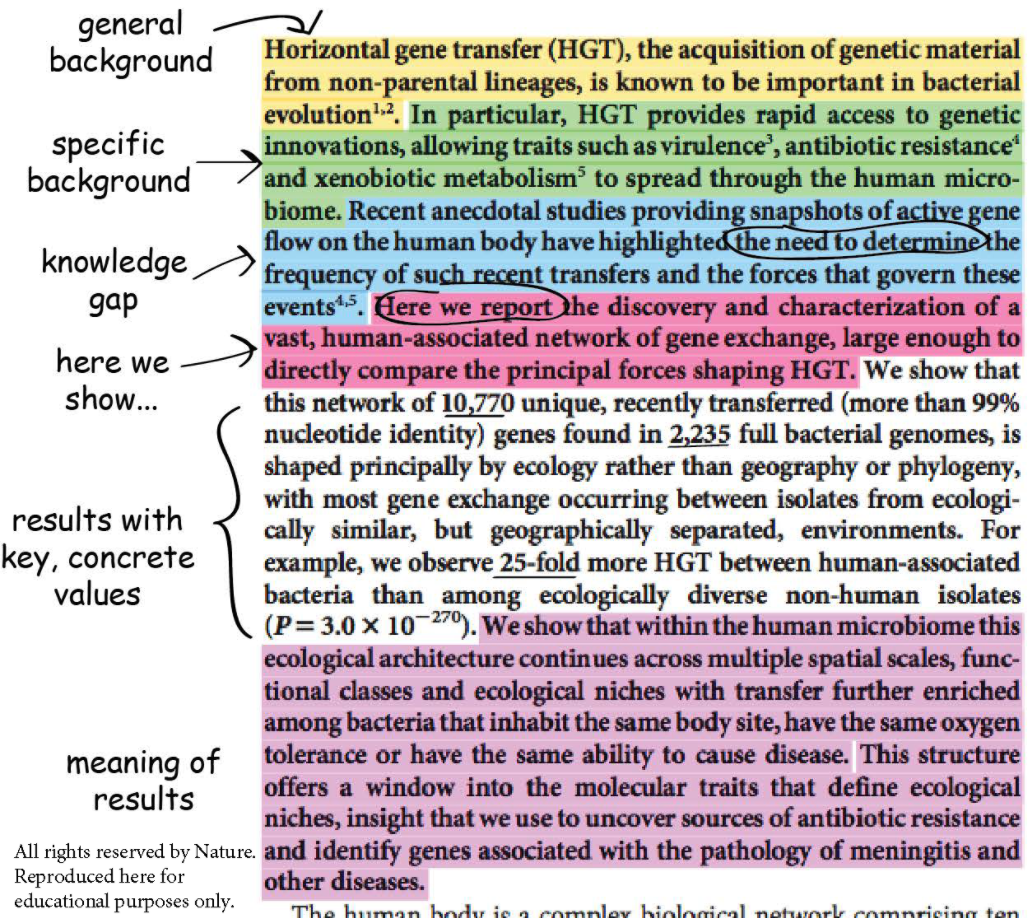
\includegraphics[width=10cm,height=10cm]{good-abstract.png}

%\afterpage{\blankpage}


\afterpreface





%%%%%%%%%%%%%%%%%%%%%%%%%%%%%%%%%%%%%%%%%%%%%%%%%%%%%%%%%%%%%%%%%%
%
% Now we can start on the first chapter
% Within chapters we have sections, subsections and so forth
%
%%%%%%%%%%%%%%%%%%%%%%%%%%%%%%%%%%%%%%%%%%%%%%%%%%%%%%%%%%%%%%%%%%



%%%%%%%%%%%%%%%%%%%%%%%%%%%%%%%%%%%%%

%\afterpage{\blankpage}


\chapter{Introduction}\label{introduction}

\section{Dossier d'ouverture}\label{dossier-douverture}

\bigskip

Au cours des dernières années, la criminalité organisée est devenue un
enjeu majeur à l'échelle internationale. Les différences observées entre
les pays en termes de taux de criminalité soulèvent des interrogations
quant aux facteurs pouvant expliquer ces variations. Parmi ces facteurs,
les conditions socio-économiques telles que le niveau de revenu, le
chômage ou encore les inégalités sociales semblent jouer un rôle
déterminant.

\medskip

Dans le cadre de ce projet, Narjis, Kawthar, Myriam ainsi que Younes ont
été missionnés par INTERPOL (a modifier si plagiat) afin de mener une
enquête sur les causes de la criminalité à l'échelle mondiale. Cette
mise en situation permet d'aborder l'analyse de manière concrète, en
mobilisant des données réelles pour répondre à une problématique
actuelle.

\bigskip

\begin{center}

\textbf{Dans quelle mesure les facteurs socio-économiques influencent-ils le taux de criminalité organisée entre pays a l'échelle l'internationale ?}

\end{center}
\medskip

\justifying

Cette question est particulièrement importante pour les décideurs
publics et les organisations internationales, car une meilleure
compréhension de ces relations pourrait permettre de mettre en place des
politiques de prévention plus efficaces et adaptées aux réalités de
chaque pays.

\medskip

Ce projet s'inscrit dans le cadre des enseignements de bases de données
(TE43MI) et de sciences des données (TE44MI). Il repose sur l'analyse de
différentes bases de données afin d'identifier les facteurs explicatifs
de la criminalité et d'évaluer leur impact.

\newpage

\section{Responsabilités et composition de l'équipe de
recherche}\label{responsabilituxe9s-et-composition-de-luxe9quipe-de-recherche}

\medskip

\begin{longtable}[]{@{}
  >{\raggedright\arraybackslash}p{(\linewidth - 4\tabcolsep) * \real{0.3056}}
  >{\raggedright\arraybackslash}p{(\linewidth - 4\tabcolsep) * \real{0.2500}}
  >{\raggedright\arraybackslash}p{(\linewidth - 4\tabcolsep) * \real{0.4444}}@{}}
\toprule\noalign{}
\begin{minipage}[b]{\linewidth}\raggedright
Nom
\end{minipage} & \begin{minipage}[b]{\linewidth}\raggedright
Statut et id
\end{minipage} & \begin{minipage}[b]{\linewidth}\raggedright
Missions principales
\end{minipage} \\
\midrule\noalign{}
\endhead
\bottomrule\noalign{}
\endlastfoot
ABBASSI Younes & Étudiant n°22401320 & Responsable de la table PAYS
(création, harmonisation, contrôles SQL) et co-responsable des analyses
descriptives R sur la répartition des pays. \\
ALLAALI Narjis & Étudiante n°22313109 & Responsable de la table
INDICATEURS année 2 et des comparaisons temporelles (SQL + préparation
des données) et co-responsable des analyses R comparatives. \\
BOUGUIMA Kawthar & Étudiante n°22303487 & Responsable de la table
CRIMINALITÉ et de la table finale d'analyse (jointures SQL) et
co-responsable des analyses R (corrélations et régressions). \\
TAGHNAKT Myriam & Étudiante n° & Responsable de la table INDICATEURS
année 1 (collecte, nettoyage, intégration SQL) et co-responsable des
analyses statistiques R et corrélations. \\
\end{longtable}

\chapter{Collecte des preuves --- Les
données}\label{collecte-des-preuves-les-donnuxe9es}

\section{Provenance des données}\label{provenance-des-donnuxe9es}

Donner ici le ou les \textbf{lien}(s) vers le(s) jeu(x) de données que
vous avez utiliser pour votre travail et présenter les rapidement.

\bigskip

Dans le jeu de données récupéré, expliquer pourquoi vous avez
sélectionné certaines tables ou pourquoi vous en avez rajouté. Vous
devez indiquer comment les données sont stockées (le format csv,
txt\ldots), la taille des fichiers, le nombre de lignes et de colonnes,
\ldots{}

\bigskip

Expliquer quels choix vous avez réalisés pour filtrer les lignes et les
colonnes (éventuellement réduire le périmètre du projet) et décrire les
critères de sélection (e.g., ne garder que 5 colonnes sur les 15, ne
garder que les lignes qui correspondent à une ville en particulier,
\ldots).

\bigskip

Finalement, définir clairement quelle est la
\textbf{population étudiée}. Vous devez expliquer quelles données vous
avez utiliser et en quoi elles peuvent permettre d'apporter des éléments
de réponses aux questions posées. Bien définir quelles sont les
\textbf{unités statistiques}.

\section{Descriptif des tables}\label{descriptif-des-tables}

Table 2.1 : Pays (156 x 3)

\begin{longtable}[]{@{}
  >{\raggedright\arraybackslash}p{(\linewidth - 6\tabcolsep) * \real{0.2466}}
  >{\raggedright\arraybackslash}p{(\linewidth - 6\tabcolsep) * \real{0.2466}}
  >{\raggedright\arraybackslash}p{(\linewidth - 6\tabcolsep) * \real{0.2603}}
  >{\raggedright\arraybackslash}p{(\linewidth - 6\tabcolsep) * \real{0.2466}}@{}}
\toprule\noalign{}
\begin{minipage}[b]{\linewidth}\raggedright
nom\_colonne
\end{minipage} & \begin{minipage}[b]{\linewidth}\raggedright
Type
\end{minipage} & \begin{minipage}[b]{\linewidth}\raggedright
Signification
\end{minipage} & \begin{minipage}[b]{\linewidth}\raggedright
Caractéristiques
\end{minipage} \\
\midrule\noalign{}
\endhead
\bottomrule\noalign{}
\endlastfoot
id\_pays & CHAR(3) & Code ISO & Clé étrangère \\
annee & INT & Année d'enregistrement des données & Non unique \\
indice\_criminalite & FLOAT & Indice de criminalité & Allant de 1 à
10 \\
\end{longtable}

Table 2.2 : Criminalité (311 x 3)

\begin{longtable}[]{@{}llll@{}}
\toprule\noalign{}
nom\_colonne & Type & Signification & Caractéristiques \\
\midrule\noalign{}
\endhead
\bottomrule\noalign{}
\endlastfoot
id\_pays & CHAR(3) & Code ISO & Clé primaire \\
nom\_pays & VARCHAR & Nom du pays & Unique \\
region & VARCHAR & Région géographique & 19 régions \\
\end{longtable}

Table 2.3 : Indicateurs (311 x 6)

\begin{longtable}[]{@{}
  >{\raggedright\arraybackslash}p{(\linewidth - 6\tabcolsep) * \real{0.2466}}
  >{\raggedright\arraybackslash}p{(\linewidth - 6\tabcolsep) * \real{0.2466}}
  >{\raggedright\arraybackslash}p{(\linewidth - 6\tabcolsep) * \real{0.2603}}
  >{\raggedright\arraybackslash}p{(\linewidth - 6\tabcolsep) * \real{0.2466}}@{}}
\toprule\noalign{}
\begin{minipage}[b]{\linewidth}\raggedright
nom\_colonne
\end{minipage} & \begin{minipage}[b]{\linewidth}\raggedright
type
\end{minipage} & \begin{minipage}[b]{\linewidth}\raggedright
Signification
\end{minipage} & \begin{minipage}[b]{\linewidth}\raggedright
Caractèristique
\end{minipage} \\
\midrule\noalign{}
\endhead
\bottomrule\noalign{}
\endlastfoot
id\_pays & CHAR(3) & Code ISO & Clé etrangère \\
année & INT & Année d'observation & Non unique \\
PIB & FLOAT & Produit interieur brut par habitant & Valeurs positives \\
chomage & FLOAT & Taux de chomage en \% & Entre 0 et 100 \\
IDH & FLOAT & Indice de développement humain & Entre 0 et 1 \\
urbanisation & FLOAT & \% population urbaine & Entre 0 et 100 \\
\end{longtable}

\chapter{Reconstitution du système --- La base de
données}\label{reconstitution-du-systuxe8me-la-base-de-donnuxe9es}

\begin{itemize}
\item
  Le MCD décrit ***** relation désequilibrée

  \begin{figure}
  \centering
  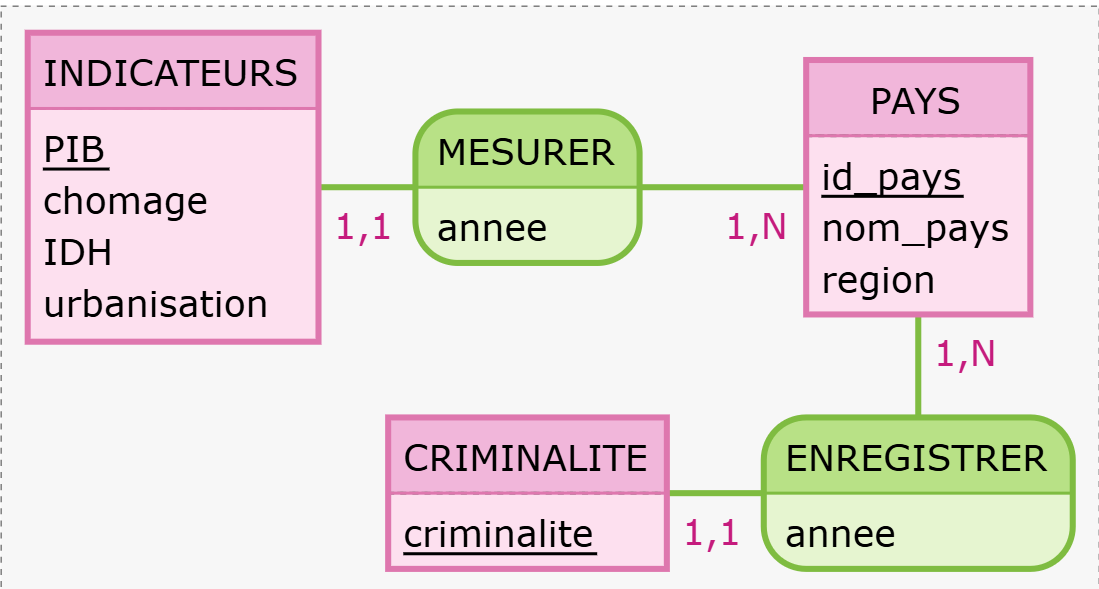
\includegraphics[width=5.20833in,height=\textheight,keepaspectratio]{res/images/uml.png}
  \caption{MCD avec Entité Pays, Criminalité et Indicateurs}\label{uml}
  \end{figure}
\item
  Le MOD

  mettre ici le diagramme phpmyAdmin
\end{itemize}

\bigskip

\section{Import des données}\label{import-des-donnuxe9es}

\begin{itemize}
\tightlist
\item
  Préciser les nettoyages réalisés avant l'import comme l'uniformisation
  des valeurs des champs (\emph{e.g.}, Mr, M., Monsieur, \ldots) ou le
  remplissage des valeurs manquantes par une valeur moyenne \ldots{}
\end{itemize}

\begin{itemize}
    \item Source de données 1 :
    \begin{itemize} 
        \item Suppression des colonnes XXX, car XXX
        \item Suppression des doublons dans les colonnes XXX
        \item Filtrage en fonction de la colonne XXX, nous n'avons conservé que...
    \end{itemize}
\end{itemize}

\section{Requêtes réalisées}\label{requuxeates-ruxe9alisuxe9es}

Pour chaque requête, l'exprimer en langage naturel puis en SQL. Puis
donner le résultat obtenu (ou un extrait) et expliquer ce résultat.

L'objectif est de varier le type de requêtes et de répondre à votre
problématique initiale.

\section{Quelques détails
techniques}\label{quelques-duxe9tails-techniques}

On peut interagir avec une base de données directement depuis RMarkdown
: i.e.~requêter puis récupérer et afficher le résultat directement
depuis le .Rmd. Un fichier connexionBDD.Rmd est fourni pour donner des
exemples.

\chapter{Matériel et Méthodes}\label{matuxe9riel-et-muxe9thodes}

\section{Logiciels}\label{logiciels}

Lister tous les logiciels utilisés pour la partie statistique du rapport
(et également ceux pour gérer et communiquer entre les membres du projet
s'il y en a en particulier)

\medskip

R (ou Python) est le logiciel à privilégier pour la Science des Données.
Pour assurer une reproductibilité maximale, vous devriez utiliser R
Markdown (ou un Notebook Jupyter, et éventuellement un outil de gestion
des versions tel que \texttt{Git}), par exemple via Google Colab ou
RStudio dans les nuages. Évitez d'utiliser Word!

\bigskip

Il est de votre responsabilité de donner les versions des logiciels que
vous utilisez, ainsi que de donner des informations techniques sur
l'ordinateur qui vous a servi pour les analyses (système d'exploitation,
vitesse du processeur, etc.). Penser à fournir des citations pour les
logiciels utilisés, par exemple
\footnote{L'entrée BibTeX ajoutée dans le fichier \texttt{references.bib} a été obtenue grâce à la commande  \texttt{citation(package = "tidyverse")} tapée dans la console de R.}.

\section{Modélisation statistique}\label{moduxe9lisation-statistique}

Quels outils ou méthodes de statistiques allez-vous utiliser? Donner des
équations mathématiques s'il y a lieu et lister les éventuels
présupposés («assumptions» en anglais) que vous devez faire sur les
données afin d'utiliser ces outils ou méthodes (\emph{e.g.}, normalité,
absence de valeurs aberrantes, etc.).

Il est également bon d'indiquer quelles sont les avantages et les
limites de ces méthodes.

Vous pourrez consulter avec profit les Chapitre 11--13 du livre sur R :

\url{http://biostatisticien.eu/springeR/livreR.pdf}

\chapter{Premiers indices --- Analyse
exploratoire}\label{premiers-indices-analyse-exploratoire}

Toute étude impliquant des données doit \textbf{obligatoirement} inclure
une analyse exploratoire préalable. Celle-ci permet de mieux comprendre
l'information contenue dans les données.

Il faut produire de nombreux résumés graphiques (\emph{e.g.},
histogrammes, nuages de points, boxplots, etc.) et numériques
(\emph{e.g.}, médiane, moyenne, variance, etc.). Ainsi, il faut faire
une analyse descriptive uni- et bivariée systématique de toutes les
variables du jeu de données. Puis, il faut uniquement conserver les plus
pertinents (les autres pouvant être gardés en Annexe), c'est-à-dire ceux
qui permettront de dégager des éléments de réponse pour la question de
recherche envisagée. Chaque figure et tableau doit être commenté. Mais
il ne faut pas extrapoler et dire des choses qui ne sont pas visibles
dans ces graphiques ou tableaux. Pour chaque analyse, vous pourrez
préciser le nombre d'individus/ d'unités statistiques concernés au
total.

Vous pourrez consulter avec profit le Chapitre 9 du livre sur R :

\url{http://biostatisticien.eu/springeR/livreR.pdf}

\section{Utiliser R}\label{utiliser-r}

Il est facile d'inclure des codes R dans votre rapport, qui seront
exécutés à la volée (\emph{i.e.}, lors de la traduction de votre fichier
\texttt{Rmd} en fichier \texttt{PDF} ou \texttt{DOC}). Par exemple:

\begin{Shaded}
\begin{Highlighting}[]
\FunctionTok{boxplot}\NormalTok{(cars, }\AttributeTok{col =} \FunctionTok{c}\NormalTok{(}\StringTok{"\#5975a4"}\NormalTok{, }\StringTok{"\#cc8963"}\NormalTok{))}
\end{Highlighting}
\end{Shaded}

\begin{figure}

{\centering \includegraphics[width=7cm]{scdon2-UPV-report-template_files/figure-latex/unnamed-chunk-1-1} 

}

\caption{\label{fig:boxplots}Deux boxplots.}\label{fig:unnamed-chunk-1}
\end{figure}

\begin{Shaded}
\begin{Highlighting}[]
\FunctionTok{colMeans}\NormalTok{(cars)}
\end{Highlighting}
\end{Shaded}

\begin{verbatim}
## speed  dist 
## 15.40 42.98
\end{verbatim}

Les lignes de code ne doivent pas dépasser dans la marge de droite.
Ainsi on pourrait remplacer le chunk ci-dessous:

\begin{Shaded}
\begin{Highlighting}[]
\FunctionTok{boxplot}\NormalTok{(cars, }\AttributeTok{main =} \StringTok{"Un titre qui est vraiment beaucoup trop long et qui dépasse dans la marge de droite"}\NormalTok{)}
\end{Highlighting}
\end{Shaded}

\begin{figure}

{\centering \includegraphics[width=7cm]{scdon2-UPV-report-template_files/figure-latex/unnamed-chunk-2-1} 

}

\caption{Pas super.}\label{fig:unnamed-chunk-2}
\end{figure}

par celui-ci:

\tiny

\begin{Shaded}
\begin{Highlighting}[]
\FunctionTok{boxplot}\NormalTok{(cars, }
        \AttributeTok{main =} \StringTok{"Un titre qui est vraiment beaucoup trop long}\SpecialCharTok{\textbackslash{}n}\StringTok{ mais qui ne dépasse plus dans la marge de droite"}\NormalTok{)}
\end{Highlighting}
\end{Shaded}

\begin{figure}

{\centering \includegraphics[width=7cm]{scdon2-UPV-report-template_files/figure-latex/unnamed-chunk-3-1} 

}

\caption{Déjà mieux.}\label{fig:unnamed-chunk-3}
\end{figure}

\normalsize

où l'on a:

\begin{itemize}
\tightlist
\item
  utilisé la commande \LaTeX~\texttt{\textbackslash{}tiny} pour changer
  la taille de la police (suivi de de
  \texttt{\textbackslash{}normalsize} pour revenir à la taille normale),
\item
  mis l'instruction \texttt{main\ =\ ...} sur la deuxième ligne,
\item
  utilisé \texttt{\textbackslash{}n} pour afficher le titre sur deux
  lignes.
\end{itemize}

\vspace{3em}

\textbf{Remarques} : Contrairement aux graphiques précédents, nous vous
demandons, pour effectuer les graphiques, d'utiliser le package
\texttt{ggplot2}. Voir
\url{https://juba.github.io/tidyverse/08-ggplot2.html} pour une courte
introduction.

\chapter{Mise à l'épreuve ---
Modélisation}\label{mise-uxe0-luxe9preuve-moduxe9lisation}

Dans cette partie, vous pourrez utiliser les outils et méthodes vus au
semestre précédent pour analyser les liens entre les variables.

Pour cela, vous pourrez utiliser les tests du \(\chi^2\), test du
coefficient de corrélation linéaire, test d'Anova, la droite de
régression linéaire.

Vous pourrez également proposer des modèles pour faire du clustering
(k-means, CAH), de la classification (K plus proches voisins par
exemple) comme vu en Science des données 1.

\section{La droite de régression linéaire : un premier
exemple}\label{la-droite-de-ruxe9gression-linuxe9aire-un-premier-exemple}

Si on souhaite expliquer les variations d'une variables réponse \(Y\) en
fonction d'un certain nombre de prédicteurs \(x_1,\ldots,x_p\), on peut
utiliser un modèle de régression linéaire simple (\(p=1\)) ou multiple
(\(p>1\))

\[
Y_i = \beta_0 + \beta_1 x_{1i} + \cdots +\beta_p x_{pi} + \epsilon_i, \qquad i=1,\ldots,n.
\] où l'on présuppose que les \(\epsilon_i\) sont i.i.d.~\(N(0,1)\) pour
tout \(i=1,\ldots,n\) (\(n\) étant la taille de l'échantillon).

Vous pourrez toujours consulter avec profit les Chapitre 11--13 du livre
sur R :

\url{http://biostatisticien.eu/springeR/livreR.pdf}

Ces chapitres détaillent l'utilisation de certains tests et modèles sous
\texttt{R}.

\chapter{Interprétation --- Résolution de
l'enquête}\label{interpruxe9tation-ruxe9solution-de-lenquuxeate}

Placer les résultats que vous avez obtenus dans le chapitre précédent en
perspective par rapport au problème étudié.

\chapter{Conclusion --- Verdict}\label{conclusion-verdict}

Quelles sont les conclusions principales? Quelles sont vos
recommandations pour le commanditaire? Quelles analyses subséquentes
pourraient être faites dans le futur?

\bigskip

On attend de vous deux types de perspectives : des perspectives à court
terme pour améliorer rapidement votre approche et des perspectives à
plus long terme qu'elles soient liées à la science des données ou au
domaine métier pour lequel vous avez travaillé.

\bigskip

Lister également les difficultés rencontrées dans la partie BD (e.g.,
taille de la base, manque de données, \ldots) et dans la partie
statistique.

\chapter*{Bibliographie}\label{bibliographie}
\addcontentsline{toc}{chapter}{Bibliographie}

\phantomsection\label{refs}

\bibliographystyle{elsarticle-harv}
\bibliography{references}

\chapter*{Annexes}\label{annexes}
\addcontentsline{toc}{chapter}{Annexes}

Il faut utiliser les annexes de façon judicieuse. C'est ici que l'on
place des résultats trop volumineux pour apparaître dans le corps du
rapport. Ou bien des résultats (e.g., graphiques) moins intéressants que
les autres. Cela permet de limiter le nombre de pages du coeur du
rapport, et d'ajouter des détails dans cette partie pour le lecteur
désireux d'en savoir plus.

\section*{\texorpdfstring{\textbf{Codes}}{Codes}}\label{codes}
\addcontentsline{toc}{section}{\textbf{Codes}}

Ajouter vos codes informatique ici. Les codes doivent être correctement
indentés et commentés.

\section*{\texorpdfstring{\textbf{Tables}}{Tables}}\label{tables}
\addcontentsline{toc}{section}{\textbf{Tables}}

Si vous avez des tableaux supplémentaires, vous pouvez les ajouter ici.

Utiliser \url{https://www.tablesgenerator.com/markdown_tables} pour
créer des tables Markdown simples, ou bien utiliser \LaTeX.

\begin{enumerate}
\def\labelenumi{\arabic{enumi}.}
\tightlist
\item
  Table Markdown
\end{enumerate}

\begin{longtable}[]{@{}lcr@{}}
\caption{une légende au-dessus du tableau.
\label{tab7.1}}\tabularnewline
\toprule\noalign{}
Les tables & sont & cool \\
\midrule\noalign{}
\endfirsthead
\toprule\noalign{}
Les tables & sont & cool \\
\midrule\noalign{}
\endhead
\bottomrule\noalign{}
\endlastfoot
col 1 est & alignée à gauche & \$1600 \\
col 2 est & centrée & \$12 \\
col 3 est & alignée à droite & \$1 \\
\end{longtable}

Aligner les nombres de la troisième colonne sur la droite permet
d'afficher les unités au-dessus des unités, les dizaines au-dessus des
dizaines, etc. Il faut toujours privilégier cette présentation.

\vspace{3em}

\begin{enumerate}
\def\labelenumi{\arabic{enumi}.}
\setcounter{enumi}{1}
\tightlist
\item
  Table Latex
\end{enumerate}

\begin{table}[h]
\centering
\caption{une légende au-dessus du tableau}
\label{tab7.1}
\begin{tabular}{lcr}
\hline
Les tables & sont & cool \\
\hline
col 1 est & alignée à gauche & 1600 \\
col 2 est & centrée & 12 \\
col 3 est & alignée à droite & 1 \\
\hline
\end{tabular}
\end{table}

\textbf{Remarques}

\begin{itemize}
  \item \{lcr\} : gauche (l), centré (c), droite (r)
  \item \verb|\caption| place la légende au-dessus
  \item \verb|\label| permet de référencer le tableau (\verb|\ref{tab7.1}|)
  \item Les nombres sont bien alignés à droite dans la 3\ieme{} colonne
\end{itemize}







\end{document}

